\documentclass[fyp]{socreport}
\usepackage{hyperref}
\usepackage{graphicx} % to insert images
\usepackage{float}
%%% code block setups
\usepackage[newfloat]{minted}
\usepackage{xcolor} % to access the named colour LightGray
\definecolor{LightGray}{gray}{0.9}
\usepackage{caption}
\newenvironment{code}{\captionsetup{type=listing}}{}
\SetupFloatingEnvironment{listing}{name=Code}
%%% code block setups
\usepackage{fullpage}

\begin{document}
\pagenumbering{roman}
\title{Competition Platform for AI Tasks}
\author{Tan Yuanhong}
\projyear{2021/22}
\projnumber{H247080}
\advisor{Dr. Akshay Narayan, Prof. Leong Tze Yun}
\deliverables{
	\item Report: 1 Volume
	\item Source Code: 1 Git Repository}
\maketitle
\begin{abstract}
TO-DO

\begin{project-nature}
	Implementation, Experimentation, Simulation
\end{project-nature}
\begin{keywords}
    \item Artificial Intelligence
	\item Machine Learning
\end{keywords}
\begin{implement}
	Ubuntu 20.04, Python 3.8, Django 4.0
\end{implement}
\end{abstract}

% \begin{acknowledgement}
%   I would like to thank my friends, families and advisors.
%   Without them, I would not have be able to complete this project.
% \end{acknowledgement}

% \listoffigures 
% \listoftables
\tableofcontents 

\chapter{Introduction}
With the increasing popularity in both artificial intelligence (AI) research and industry application, more and more institutions are considering AI education as an integral part of their computer science or even general education curriculum. However, in spite the algorithmic nature of AI education, there is surprisingly few platforms and tools to host AI competitions/assignments and automatically grade the submissions. Unlike traditional algorithm and data structure courses that have many online judges available (to name a few, \href{https://codeforces.com/}{Codeforces}, \href{https://open.kattis.com/}{Kattis}, \href{https://onlinejudge.org/}{UVa Online Judge}), AI courses often rely on arbitrary grading scripts or in-house solutions to host their assignments/contests. There are well-known data science competition platforms like \href{https://www.kaggle.com/}{Kaggle} that are suitable for prediction/classification tasks, but the area of reinforcement learning (RL) tasks \footnote{To be precise, here tasks mean environments that are typically used for RL algorithms. The differentiating characteristic of such tasks is that they are interactive (in contrast to comparing the output against the ground truth like what Kaggle and other traditional OJs do).} remains surprisingly untouched. Therefore, this project tries to fill the gap of evaluating algorithms that solve interactive tasks. We aim to provide a complete solution from building RL \footnote{Technically the evaluation model we use is suitable for almost all AI/ML tasks (including classification and regression), but we will focus on RL first since we already have Kaggle for classification/regression tasks.} environments, writing test cases, to eventually hosting these tasks on a massively scalable platform.

\section{Problem Statement}
In this section, we briefly discuss the history and background
of the problem.  A detail literature survey is presented in 
Chapter \ref{ch:related}.

\chapter{Literature Review}
\label{ch:related}
\section{Background}
\subsection{Reinforcement Learning Tasks}
Reinforcement learning (RL) is a branch of machine learning that maps observations (possibly with history as well) to actions such that certain metrics are maximized \cite{sutton-barto}. The metrics which agents try to maximize are called a reward or reinforcement, thus the name “reinforcement” learning. In a broader sense, any AI task is RL task: we can generalize any input as the observation, any output as the action and any target as the reward. But for the sake of simplicity, in this report, by RL task we mean sequential decision problems (SDP), where the outcome of agent’s decision depends on a sequence of decisions \cite{russell}.

A sequential decision problem is fully described by state space, action space, transition model and a reward function \cite{russell}. A transition model is a function that maps (current state, history states, action) to a probability of reaching any possible state. If the transition model does not depend on history state, we call it Markovian as the probability only depends on the current state instead of the history of all earlier states. A reward function maps current state \footnote{Reward function may also depend on action and next state, but one that only depends on the current state is the most common variant, and this difference is not fundamental.} to a numerical reward.

The solution to a sequential decision problem is called a policy. It is a function that maps current state (and sometimes history states) to an action. We always assume that the domain of policy function is the entire observation space so that the agent knows what action to take under any possible circumstance. The goal of RL algorithms is to come up with such policy functions that maximize their expected reward under different settings (e.g., unknown underlying transition model, partial observability, etc.).

From the definition of sequential decision problems, we can summarize the following execution loop of any typical SDP:

\begin{figure}[htp]
    \centering
    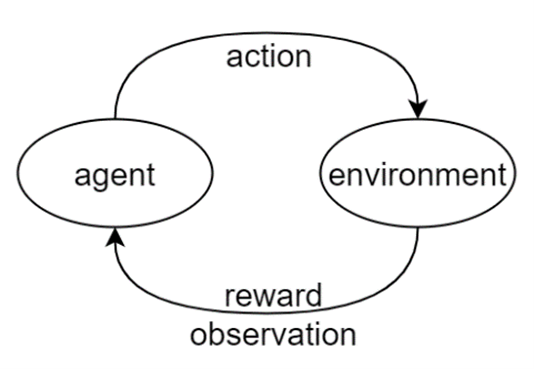
\includegraphics{images/obr-loop.png}
    \caption{Action-observation-reward loop}
    \label{fig:obr-loop}
\end{figure}

In other words, the environment implements the transition model $P\left(s_j\middle| s_i,a\right)$ and reward function $r\left(s_i\right)$ and returns the next observation $o_j$ and reward $r_j$ to the agent, after which the agent takes another step of action $a_{j+1}$ based on $\left[o_j,o_{j-1},\cdots,o_0\right]$ and $\left[r_j,r_{j-1},\cdots,r_0\right]$. Note that $o_i$ and $s_i$ may or may not be the same depending on whether the environment is fully observable.

\subsection{Reinforcement Learning Environment Frameworks And Collections}
RL research, like many computer science topics, requires concretizing the theory with implementation and experiments as they are equally important. That is where RL environment frameworks and collections like the Arcade Learning Environment (ALE) \cite{ale} and OpenAI Gym \cite{openai-gym} come into play. Such an effort is incredibly important for the rapid growth of the RL community: it not only saves researchers a lot of emulation development time, but also provides benchmark environments to evaluate RL tasks similar to how CIFAR-10 \cite{cifar-10} provides benchmark datasets in image classification. A typical OpenAI Gym agent code is structured as below:

\begin{code}
\begin{minted}[
frame=lines,
framesep=2mm,
baselinestretch=1.2,
bgcolor=LightGray,
fontsize=\footnotesize,
linenos
]{python}
import gym

env = gym.make('CartPole-v0')
for i_episode in range(100):
    observation = env.reset()
    for t in range(100):
        action = decide(observation, reward)
        observation, reward, done, info = env.step(action)
env.close()
\end{minted}
\captionof{listing}{OpenAI Gym agent example}
\label{code:gym-agent}
\end{code}

Besides collecting many classical environments as a benchmark package, an important contribution of OpenAI Gym is its widely accepted application programming interface (API). This common interface proves to be sufficient for not only hundreds of self-contained environments included in OpenAI Gym, but also thousands more third-party environments. When it comes to turning retro video games to RL environments, Gym dominates the game by eventually having ALE adopt its API and merge into Gym. Moreover, as if conquering Atari2600 is not enough, Gym Retro \cite{gym-retro} adds even more emulated systems such as Nintendo Game Boy and Sega Genesis to Gym. Therefore, it is safe to say that following this interface gives us enough flexibility to implement most of the desired environments.

From the source code of OpenAI Gym, a compatible environment needs to implement the methods and attributes shown in Figure \ref{fig:gym-class}:

\begin{figure}[htp]
    \centering
    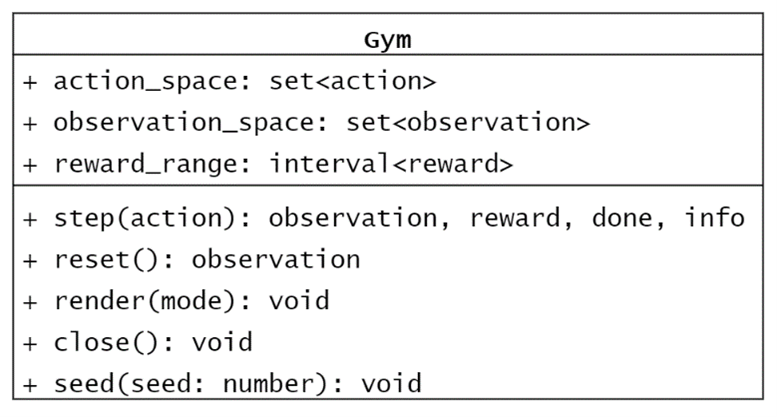
\includegraphics{images/gym-class.png}
    \caption{OpenAI Gym Class Diagram}
    \label{fig:gym-class}
\end{figure}

Authors of OpenAI Gym listed multi-agent as a future direction when they published the paper in 2016. However, as of 2021, there is still no official support for multi-agent tasks. There are some third-party environments that support multi-agent tasks, like ma-gym \cite{magym}. These implementations usually convert multi-agent observation, reward, and action into a vector, length of which is equal to the number of participating agents in the environment.

\section{Related Work}

\subsection{Online Judging System}
Online judges first emerged to address the problem of automatically grading programming assignments conveniently, fairly and securely \cite{RN4}. Without any manual intervention once the system is configured properly, online judge systems need to handle 1) receiving submissions, 2) compiling and executing source codes, 3) comparing outputs against the correct answers, 4) logging the result. For fairness, RAM and CPU usage will be monitored and limited. Usually, there is a hard time limit after which any submission will be forced to terminate. For security, execution of arbitrary submission needs to be contained in a safe environment with heavily restricted privilege levels such that only necessary operations are allowed, any other attempt (e.g., accessing the network, read/write on filesystem, etc.) will be blocked and preferably reported to the system administrator. 

Among all the challenges in building a successful online judge, security is probably the most technically difficult aspect. Some online judges were used in an exam setting where students had to use dedicated terminals for access, and a system administrator is involved in monitoring the security issues \cite{10.1145/384267.305835}. For automated security measures, there are generally two approaches: 1) source code or binary scanning, and 2) operating system level access control. 

Source code or binary scanning has no runtime performance penalty, but it requires an exhaustive check on all possible malicious tokens/system calls. It is unrealistic to have a perfectly secure source code scanner and every new supported language \footnote{A “new” language does not have to be a completely new one. If new keywords or new compiler version is introduced, there could possibly be new security implications.} requiring a new set of scanning rules makes this approach non-sustainable \cite{RN4}. Besides, it is impossible to scan the binary for programs written in a dynamic programming language such as Python as they execute inside an interpreter.

Access control based on operating system kernel security features is much more foolproof and widely applicable. Such techniques are also called OS-level virtualization because from the perspective of programs inside a “namespace”, it can only see partial filesystem and devices that are assigned to this “namespace”. Since the introduction of user namespaces in Linux kernel 3.8, containerization technology has become increasingly popular to provide isolation between processes while being able to share nearly all hardware resources with minimal performance overhead \cite{RN16}. 

With the rapid growth of cloud and distributed computing, there are also novel online judges that attempt to adopt these cutting-edge technologies. A distributed online judge architecture tries to address the problem of scalability: an online judge needs to execute student submissions, and with more students and courses, computation required grows linearly. It is difficult to scale up (making computers more powerful) but easy to scale out (having more computers) especially in recent years with the emergence of cloud computing \cite{RN17}. Evaluating AI tasks has an even stronger demand for horizontal scalability as neural networks or sophisticated searching algorithms are notoriously computationally heavy. Notable implementations of distributed online judge include MetaOJ \cite{metaoj}, which separates data storage, web application and judgers into three separate components that can be deployed to the cloud independently (Figure \ref{fig:metaoj}).

\begin{figure}[H]
    \centering
    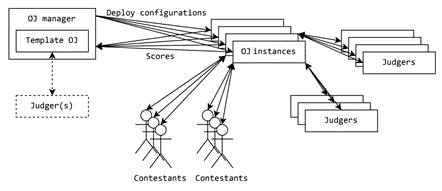
\includegraphics{images/metaoj.png}
    \caption{MetaOJ architecture}
    \label{fig:metaoj}
\end{figure}

\subsection{ML/RL Benchmark Platforms}
In contrast to competition platforms on the education side, researchers are more interested in a benchmark platform that provides a collection of tasks to compare different RL algorithms. Such benchmarks are crucial for reproducible and verifiable research in RL. According to Vanschoren and Blockeel (2009), an interpretable and reproducible experiment consists of four parts: algorithm, parameters, evaluation method and dataset. For a benchmark, evaluation method and dataset are fixed while contributors will compare different algorithms and parameters. In the context of RL benchmark, this means packaging the simulation environment and evaluation metrics behind a simple set of common interfaces for both training and testing.

\chapter{Problem and Algorithm}

\chapter{Evaluation}

\chapter{Conclusion}

\bibliographystyle{socreport}
\bibliography{socreport}

\appendix
\chapter{Code}

% \chapter{Proofs}
% In this appendix, we present alternate, longer, but more interesting proof 
% of correctness of our algorithm.  This proof is based on induction and proof
% by contradiction.
\end{document}
